\documentclass [10pt,letterpaper]{report}
%\documentclass[10pt,letterpaper]{article}
%\documentclass[10pt,letterpaper,twocolumn]{article}
%
%\documentclass[10pt,letterpaper,twocolumn]{report}
%\documentclass[10pt,letterpaper]{report}
%
%\usepackage[greek,english]{babel}
\usepackage[greek,english]{babel}
\usepackage[T1]{fontenc}
\usepackage{graphicx}
\usepackage{color}
\usepackage{wrapfig}


\textheight     =   8.4in
\textwidth      =   6.8in
%\parindent     =   0.0cm

\topmargin      =  -0.2in
\oddsidemargin  =  -0.2in
\evensidemargin =  -0.2in
%\hoffset       =   0.0cm
%\voffset       =   0.0cm

\newcommand{\nuSolve}{\greektext n\latintext Solve}
\newcommand{\thisVersion}{0.5.2}

\graphicspath{{graphics/}}

\begin{document}

\title{vgosDbCalc-\thisVersion{}: User Guide}

\author{
Sergei Bolotin,
Karen Baver,
John Gipson,
David Gordon,
Daniel MacMillan
}

\date{\today}


\maketitle

\tableofcontents


\def\leftSp      {48mm}
\def\riteSp     {113mm}


\chapter{Introduction}
\label{intro}

This document describes how to use the utility vgosDbCalc.

The utility performs calculating of theoretical values and their partials
with respect to estimated parameters. It consists of two parts: the legacy
software CALC (of the current version) and a replacement of the old database
I/O library by the new one that deals with vgosDb format.

The utility vgosDbCalc is distributed in nusolve package that contains \nuSolve{}
software and utilities vgosDbMake, vgosDbCalc and vgosDbProcLogs. Each of the
utilities has its own version number that can differ from distribution version,
e.g., the first release of vgosDbCalc-0.1.0 appeared in nusolve-0.4.0 package.

The guide covers \thisVersion{} version of the software. Since the vgosDbCalc
is a simple utility we do not expect large modifications of the
User Guide version from version.



%
%
%
\section{Requirements}
\label{intro_reqs}

See \emph{\nuSolve{} User Guide} for the requirements.


%
%
%
\section{Changes from previous versions}
\label{intro_changes}

This section was added in 0.5.0 version of the nusolve distribution (version 0.2.0
of the vgosDbCalc User Guide). It covers changes in the software and the user guide.


\subsection{Changes in version 0.5.3}
No significant changes in this version were done.

\subsection{Changes in version 0.5.2}
The section \emph{\ref{config_paths} Setting paths to data} was updated to reflect
changes in master file handling and a new option to load only wrapper files that were
produced by local analysis center.



\subsection{Changes in version 0.5.1}
Nothing essential was changed.

\subsection{Changes in version 0.5.0}
Sources of CALC and nusolve are decoupled. To compile vgosDbCalc a user have to
install libCalc first. The sources of vgosDbCalc now does not contain CALC codes.
As a result, configuration, compiling and installation of vgosDbCalc is much easier,
no specific options are necessary. In the case if libCalc is missing, the utility
will not be configured and compiled. At the time of writing libCalc is available at
\begin{center}
{\tt
https://sourceforge.net/projects/libcalc/
}
\end{center}

Support of version 2 of masterfile and new database naming convention is added.

\subsection{Changes in version 0.4.6}
Nothing essential was changed.

\subsection{Changes in version 0.4.5}
Nothing essential was changed.


\subsection{Changes in version 0.4.4}
The command line arguments parser has switched to ARGP from GNU C Library.

A bug that prevents reading a database by session name if only one wrapper file
exists (usually when vgosDbCalc is running) was found and fixed.


\subsection{Changes in version 0.4.3}
Instructions on installation of the software was moved to \nuSolve{} User Guide.
Chapter \emph{\ref{chapter_installation} Installation} was modified to reflect the changes.


\subsection{Changes in version 0.4.2}
Nothing essential was changed.


\subsection{Changes in version 0.4.1}
Nothing essential was changed.


\subsection{Changes in version 0.4.0}
New command line arguments were added, see the chapter
\emph{\ref{chapter_invokation} Invoking vgosDbCalc} for details.

A dry mode has been implemented, the software reads input files, creates and fills
all internal structures, but nothing is written.

Dealing with locale has been altered. Unfortunately, people do not read the manuals,
as a result their locale set up conflicts with HOPS parsing of fringe files. Now,
by default the locale is set to "C" after the utility is started. There are options
to configure this feature in the wizard as well as a command line argument.


\subsection{Changes in version 0.3.4}
Nothing essential was changed.

\subsection{Changes in version 0.3.3}
This update contains bug fixes.

\subsection{Changes in version 0.3.2}
In this version behavior of vgosDbCalc has been modified: if the environment
variable <<\$DISPLAY>> is not set, calls to pop up windows with error messages are
suppressed. Also, during creation of the wrapper file name, the attribute
<<\_i[Institution]>> will be added. To suppress the last option, the short
abbreviation of the affiliation should not be set (e.g., on the Fig.~\ref{fig-wizzard-3}
put an empty string instead of <<GSFC>>).

A warning about permanently increase of the log file size was added to the section
\emph{\ref{config_logger} Setting options of the logger}.

A notion about locale configuration of the shell environment have been
added to the chapter \emph{\ref{chapter_invokation} Invoking vgosDbCalc}.


\subsection{Changes in version 0.3.1}
The command line options {\tt -p} and {\tt -W} are added in this version, see
the chapter \emph{\ref{chapter_invokation} Invoking vgosDbCalc}.

A section \emph{\ref{sect_systemwide_settings} Using system-wide settings} is added.

The URL of software distribution has been updated in the chapter
\emph{\ref{chapt_concluding_remark} Concluding remark}.


\subsection{Changes in version 0.3.0}
Several bug fixes were made in vgosDbCalc.
The version of the user guide was updated to be compatible with the version of the
utility.

\subsection{Changes in version 0.2.0}
The utility is able to read an alternative version of master files. The
use of the local master files is described in the section
\emph{\ref{config_paths} Setting paths to data}.

The sections \emph{\ref{intro_reqs} Requirements} and
\emph{\ref{intro_changes} Changes from previous versions} were added to
the chapter \emph{\ref{intro} Introductions}.








%%%%%%%%%%%%%%%%%%%%%%%%%%%%%%%%%%%%%%%%%%%%%%%%%%%%%%%%%%%%%%%%%%%%%%%%%%%%%%
%
%
\chapter{Installation}
\label{chapter_installation}

The source codes of vgosDbCalc is distributed along with \nuSolve{}
software. The latest stable version of the software one can find at
{\tt https://sourceforge.net/projects/nusolve} with a name like
{\tt nusolve-1.2.3.tar.gz}. Since the software is still in an active
development phase, we recommend you use the latest version.

The utility is compiled during compilation of \nuSolve{} software. Please
refer to \nuSolve{} User Guide how to configure, compile and install the
software.

%
%However, there is a trick in installation of vgosDbCalc that arises from
%CALC part of software. Paths and file names of some a priori data are
%hard coded in CALC and need to be adjusted before compilation. The file
%{\tt src/vgosDbCalc/calc11/param11.i} contains the following parameters
%that needs to be checked:
%\begin{verbatim}
%JPL_DE421
%OPTL_file
%DFLEAP
%\end{verbatim}
%The a priori files for CALC use are in {\tt data} directory of the nusolve
%distribution. Put them to some place and adjust the file {\tt param11.i} to
%tell CALC where they are.
%





%%%%%%%%%%%%%%%%%%%%%%%%%%%%%%%%%%%%%%%%%%%%%%%%%%%%%%%%%%%%%%%%%%%%%%%%%%%%%%
%
%
\chapter{Invoking vgosDbCalc}
\label{chapter_invokation}
To invoke vgosDbCalc just type (specifying if necessary the full path
to the executable) program name and a wrapper file of a VLBI session:
\begin{verbatim}
> vgosDbCalc <wrapper file>
\end{verbatim}
\noindent
The utility also accepts command line arguments. The arguments consist of
two groups of options and a name of alternative configuration. The first
group of options is related to Qt library and controls how the application
will appear and behave. See Qt documentation about details, (e.g.,
https://doc.qt.io/qt-5.14/qguiapplication.html).
%http://qt-project.org/doc/qt-4.8/qapplication.html\#QApplication).
The another group of options is used by itself. To get the list
of these arguments, type

\begin{verbatim}
> vgosDbCalc --help
\end{verbatim}
\noindent
Here are command line arguments that are available at the time of writing:
\vspace{5mm}

\begin{tabular}{p{\leftSp}p{\riteSp}}
\multicolumn{2}{c}{General options:}\\
{\tt -l, -{}-std-locale}        & Use the standard locale.\\
\end{tabular}
\vspace{5mm}

\begin{tabular}{p{\leftSp}p{\riteSp}}
\multicolumn{2}{c}{Configuration control:}\\
{\tt -a, -{}-alt=STRING}        & Use an alternative configuration STRING.\\
\end{tabular}
\vspace{5mm}

\begin{tabular}{p{\leftSp}p{\riteSp}}
\multicolumn{2}{c}{Invocation of startup wizard:}\\
{\tt -w, -{}-wizard}            & Force call of the startup wizard.\\
{\tt -W, -{}-sys-wide-wizard}   & Run startup wizard for the system-wide settings.\\
\end{tabular}
\vspace{5mm}

\begin{tabular}{p{\leftSp}p{\riteSp}}
\multicolumn{2}{c}{Operation modes:}\\
{\tt -?, -{}-help}              & Give this help list.\\
{\tt -p, -{}-print-setup}       & Print set up and exit.\\
{\tt -q, -{}-dry-mode}          & Process in a "dry run" mode: files will not be created, instead names of the files will be printed.\\
{\tt     -{}-usage}             & Give a short usage message.\\
{\tt -V, -{}-version}           & Print program version.\\
\end{tabular}
\vspace{5mm}


\noindent
Most of these options are used either to override the current software configuration
or for the debug purposes.

An alternative to providing the name of a wrapper file could be specifying
a database name or a database name and version number. For example, running
vgosDbCalc for a VLBI session EUROPE-136 which is stored in a database 15AUG03XA
can be done using a master file name
\begin{verbatim}
> vgosDbCalc /home/slb/500/vgosDb/2015/15AUG03XA/15AUG03XA_V001_kall.wrp
\end{verbatim}
or a database name can be provided to vgosDbCalc instead of the mater file name
\begin{verbatim}
> vgosDbCalc 15AUG03XA_V001
\end{verbatim}
If a user wants to process a wrapper file with the last version, the version suffix
can be omitted:
\begin{verbatim}
> vgosDbCalc 15AUG03XA
\end{verbatim}


The command line argument <<-l>> preserve altering of the locale. If you want to
use this option,
please check locale setting of your shell environment.
CALC software uses libC functions that are locale aware.
Different languages have different rules for string comparison,
representation of integer and real numbers and so on, so using locale other
than standard "C", "POSIX" or "en" could cause incorrect work of the
software. You can check your environment locale setting with command
\begin{verbatim}
> locale
\end{verbatim}
\noindent
Consult with your system administrator for details.





%%%%%%%%%%%%%%%%%%%%%%%%%%%%%%%%%%%%%%%%%%%%%%%%%%%%%%%%%%%%%%%%%%%%%%%%%%%%%%
%
%
\chapter{Configuring the software}
\label{chapter_configuration}
When vgosDbCalc is invoked the first time or new alternative
configuration name has been provided, it calls a setup wizard. The
wizard is a small application that asks a user few questions about the
configuration.

If you want to change your current configuration, run vgosDbCalc with
{\tt -w} option:
\begin{verbatim}
> vgosDbCalc -w
\end{verbatim}
\noindent
If you want to set up (or change) the configuration of alternative setup,
invoke vgosDbCalc with {\tt -a AltCfg} option. For example, executing
\begin{verbatim}
> vgosDbCalc -w -a Test
\end{verbatim}
will create an alternative set up under the name {\tt Test}. To use this
set up invoke vgosDbCalc as
\begin{verbatim}
> vgosDbCalc -a Test <wrapper file>
\end{verbatim}
A name of an alternative setup should not contain {\tt <</..>>} sequence of chars.



\section{Using system-wide settings}
\label{sect_systemwide_settings}
On a system with several users it is useful to set up common software settings,
like path to observations, data files, and so on. To set up such settings, invoke
the utility with {\tt -W} option. Obviously, you have to have write access to the
directory with system-wide settings. By default, the system-wide settings directory
is derived from {\sl \$\{prefix\}} variable of the {\tt configure} script and is
set to {\sl \$\{prefix\}/etc/xdg}. It can be overwritten using {\sl --sysconfdir}
option of the {\tt configure} script.

The system-wide settings take an effect if user settings do not exist (e.g., first
run of the software), they do not change existing user's settings.

Combination of the option {\tt -W} with the option {\tt -a AltCfg} discards
using the system-wide settings, the setup wizard will use the alternative setup
instead.

Due to a problem in implementation of QSettings object, the system-wide settings
option is available only if you have Qt library of version 4.8.0 or newer.


\section{Setting paths to data}
\label{config_paths}
On the first after the introduction wizard's page, "Home directory", user can
set up paths to the default directories. The directory set up is similar to
configurations of vgosDbMake and vgosDbProcLog utilities.

The home directory of vgosDbCalc is a place where all non-absolute (i.e., a path
that does not start with "/" character) paths refer to.

\begin{figure}[htb!]
  \begin{center}
    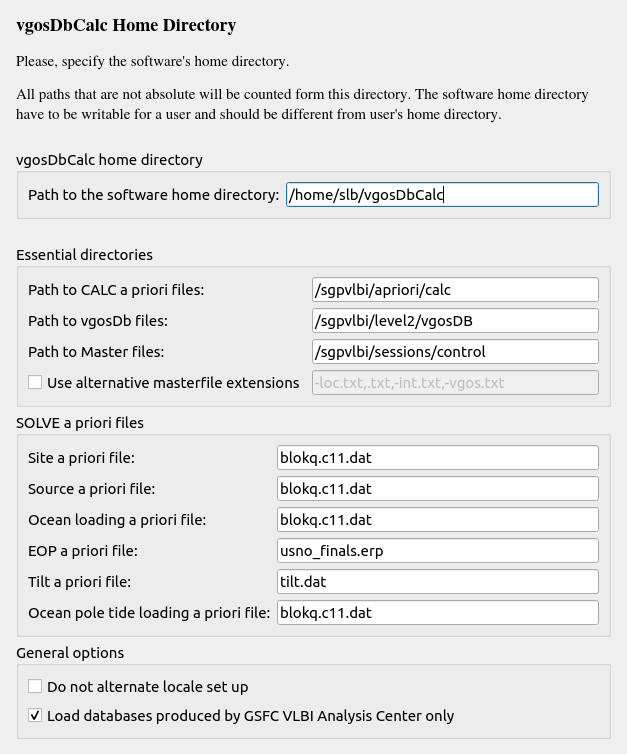
\includegraphics[width=0.6\textwidth]{wz-1-calc.jpg}
  \end{center}
  \caption{Setting up paths.}
  \label{fig-wizzard-1}
\end{figure}

The path to CALC a priori files is in {\tt Path to CALC a priori files} filed.
The {it a priori} files are available in the distribution. However, one file
that contains ERP data (in the distribution it called {\tt usno\_finals.erp})
have to be updated time from time.

% ! https://cddis.nasa.gov/archive/vlbi/gsfc/ancillary/solve_apriori/

The path to VLBI observations in vgosDb format is specified by the field {\tt Path to vgosDb files}.
The data structure of vgosDb files would looks like
\begin{verbatim}
   <VGOSDB_ROOT>/YYYY/YYMMMDDBL/<data files>
\end{verbatim}
Where {\tt VGOSDB\_ROOT} is a directory specified in the wizard, {\tt YYYY} is
a year and {\tt YYMMMDDBL} is a database name.

The software uses master files to figure out a proper database name.
The path to the master files is a place where these files are
supposed to be. You can obtain the fresh copies of master files from
\begin{center}
{\tt
https://cddis.nasa.gov/archive/vlbi/ivscontrol
}
\end{center}
\noindent
Time from time the files need to be updated. In addition to the standard master
files, a user can use its own "local" master file. The format of the local master
file should be the same as the standard one, its name have to be in the form
"masterYY-loc.txt", where "YY" -- two digits of the year. This feature is designed
for testing purposes or processing non-standard VLBI sessions. The software first
checks for the local master files, if it found a record there it stops the search,
so records in the canonical master files can be overwritten using the local
master file.

Starting with version 0.8.2 of the distribution, an option to expilictly set names
for master files is added. If a user sets the check box {\sl Use alternative
masterfile extensions} to <<on>>, then vgosDbCalc will compose the masterfile names
using a provided list of extensions. The list is a set of strings separated by
comma (","), colon (":") or semicolon (";") char. The software adds the extension
from the list to the basic name, "masterYY" or "masterYYYY", and reads such a file.
The order of files lookup is corresponding to the order of masterfile
extensions in the list. The default list of masterfile extensions is
"-loc.txt,.txt,-int.txt,-vgos.txt".

The check box {\tt Do not alternate locale set up} controls how the utility
deals with locale set up. By default it is <<off>>.

When a user loads a vgosDb database providing a session name, vgsDbCalc
usually reads the lates version of a wrapper file of the database.
However, sometimes it is preferrable to load the latest version produced
by your analysis center even if a higher version created by another
institution already exists. In this case turn on the checkbox
{\sl Load databases produced by [local] VLBI Analysis Center only}, where
[local] is an abbreviated acronym of your analysis center (see the next subsection).






\section{Setting user identities and affiliation}
The second and third pages of the wizard, Fig.~\ref{fig-wizzard-2}-\ref{fig-wizzard-3},
set up user identities and affiliation.

\begin{figure}[htb!]
  \begin{center}
    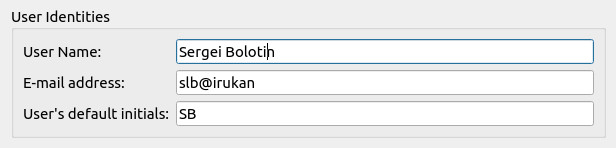
\includegraphics[width=0.6\textwidth]{wz-2-calc.jpg}
  \end{center}
  \caption{Setting up user ID.}
  \label{fig-wizzard-2}
\end{figure}

%\section{Setting affiliation}

\begin{figure}[htb!]
  \begin{center}
    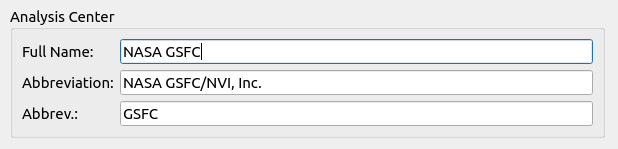
\includegraphics[width=0.6\textwidth]{wz-3-calc.jpg}
  \end{center}
  \caption{Setting up affiliation.}
  \label{fig-wizzard-3}
\end{figure}

We strongly encourage users to provide, at least, a working e-mail
address.

Information collected by these two pages are used only for composing the
history part of vgosDb files and in vgosDbCalc log file.

The short form of the abbreviated affiliation (<<Abbrev.>> on the
Fig.~\ref{fig-wizzard-3}) is used in wrapper file names as an attribute
{\sl \_i<Institution>}. If the field is empty, the attribute will not be
added to a name of a wrapper file.


\section{Setting options of the logger}
\label{config_logger}
The last page of the start up wizard, Fig.~\ref{fig-wizzard-4}, sets up
properties of the logging subsystem. The field {\tt Log file name} is
a name of a file where the log messages will be saved if the checkbox
{\tt Save log to the file} is checked <<on>>. The file will appear in
vgosDbCalc home directory, Fig.~\ref{fig-wizzard-1}. The {\tt Log capacity}
is an amount of log records that are kept in internal structure before
send them to a file. The checkbox {\tt Put time stamps} turns on
adding time tags to the log messages.

\begin{figure}[htb!]
  \begin{center}
    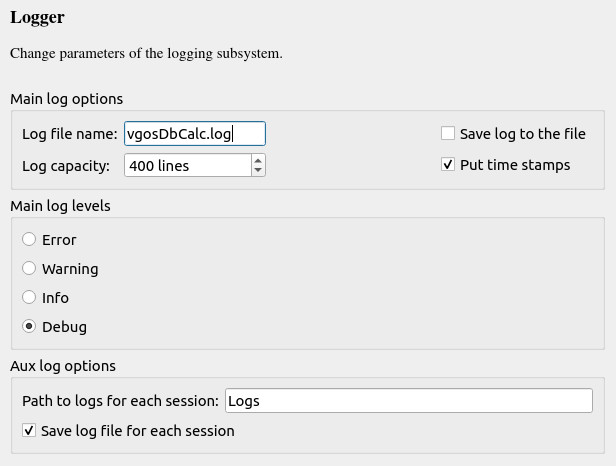
\includegraphics[width=0.6\textwidth]{wz-4-calc.jpg}
  \end{center}
  \caption{Setting up logger.}
  \label{fig-wizzard-4}
\end{figure}

The {\tt Log level} determines how verbose the log output will be. The {\tt Debug}
level, as shown on the figure, could be useful for debugging purposes. For
routine operations the {\tt Info} level will be preferred.

%The software does not control the size of the main log file, it will grow up
%with each invocation of the utility. A user should control the size of the log
%file and remove or back it up, what is necessary.

Another log file will be created on a per session basis if the checkbox
{\tt Save log file for each session} is turned <<on>>. The aux log file
will be saved in {\tt Path to logs for each session} directory and its
name will be the same as the database name plus ".log" extension.

{\bf \color{red}WARNING}: If the logger is instructed to save data in
the log file, the size of the file will grow up. The software does not
check the size of the file (it does not know about your intentions), and
eventually the file could take all free space on your computer! If you
do not need the log output from previous runs, please, remove the file on
a regular basis.



%%%%%%%%%%%%%%%%%%%%%%%%%%%%%%%%%%%%%%%%%%%%%%%%%%%%%%%%%%%%%%%%%%%%%%%%%%%%%%
%
%
\chapter{Concluding remark}
\label{chapt_concluding_remark}
Currently, this document is in the developmental stage, its content could change
time from time. Check for new versions at the ftp site:

\begin{verbatim}
      https://sourceforge.net/projects/nusolve
\end{verbatim}

\noindent
If you have questions or suggestions that will improve the software or
the User Guide, please e-mail us at:

\begin{verbatim}
      <mailto:sergei.bolotin@nasa.gov>
\end{verbatim}

%\noindent
%Happy !


%%%%%%%%%%%%%%%%%%%%%%%%%%%%%%%%%%%%%%%%%%%%%%%%%%%%%%%%%%%%%%%%%%%%%%%%%%%%%%
%
%
\begin{thebibliography}{99}

\bibitem{Bolotin2010}
S. Bolotin, J. Gipson, D. MacMillan: ``Development of a New VLBI Data
Analysis Software". In: International VLBI Service for Geodesy and
Astrometry 2010 General Meeting Proceedings, edited by D. Behrend and K.
Baver, NASA/CP-2010-215864, 197-201, 2010.


\bibitem{Bolotin2011}
S. Bolotin, J. Gipson, D. Gordon, D. MacMillan: ``Current Status of
Development of New VLBI Data Analysis Software". In: Proceedings of the
20th Meeting of the European VLBI Group for Geodesy and Astrometry,
edited by W. Alef, S. Bernhart, A. Nothnagel, Schriftenreihe des
Instituts f\"ur Geod\"asie und Geoinformation der Universit\"at Bonn,
Nr. 22, ISSN 1864-1113, 86-88, 2011.


\bibitem{Bolotin2012}
S. Bolotin, K. Baver, J. Gipson, D. Gordon, D. MacMillan: ``The First
Release of $\nu$Solve". In: International VLBI Service for Geodesy and
Astrometry 2012 General Meeting Proceedings `Launching the
Next-Generation IVS Network', edited by D. Behrend and K. Baver,
NASA/CP-2012-217504, 222-226, 2012.


\end{thebibliography}


\end{document}


